\documentclass[12pt]{article}
%\input{hw_macros.tex}

\setlength{\topmargin}{-.75in} \addtolength{\textheight}{2.00in}
\setlength{\oddsidemargin}{.00in} \addtolength{\textwidth}{.75in}

\usepackage{amsmath,color,amssymb,graphicx,esdiff}
\usepackage[shortlabels]{enumitem}
\pagestyle{empty}
\usepackage{listings}

\setlength{\parindent}{0in}
\setlist[enumerate]{leftmargin=*}
\begin{document}

{\sc {\bf {\large Homework 2}}
            \hfill {MTH 629, Fall 2021}}
\bigskip

{\bf Due Friday, Oct. 8\textsuperscript{th} by 11:59 pm on Canvas}

\section{Chapter 3}
\textbf{Problem 1}
\vspace{5pt} 

A medical lab is testing machine learning software which actively regulates oxygen levels in ventilators. If oxygen levels fall outside of an acceptable range, the ventilators automatically reset. A twenty day study is done with the response variable the time in days (eventtime) until the ventilators reset. The exposure variable, Setting, indicates whether the software is disabled (Setting=2), at the standard setting (Setting=1) or at the newly coded setting (Setting=0). The variable LO2 indicates the level of oxygen gas, compared to a baseline, that is supplied to the ventilator through a main tube.
\begin{enumerate}[i.]
\item Load the data by using the following command in R

 \lstinline{load(``Venreset.RData'')}

\item Create a survival object from the data set and call it V. In R, create three Kaplan-Meirer Curves from your data for each setting in a single plot. Add a legend to your plot. Conduct a log-rank test for the effect of the setting variable on event times. Based on the log-rank test, what conclusion can you reach about the significance of the effect on event times of the software setting?
\item In R, build three Cox PH models for the Ventilator data: 
\begin{enumerate}
\item A model that just accounts for Setting. Give the fitted Cox PH model and interpret the estimated coefficient of Setting.
\item A model that accounts for Setting and LO2.
\item A model that accounts for Setting, LO2 and interaction between Setting and LO2. Give the fitted Cox PH model.
\begin{enumerate}[1.]  
\item Give confidence intervals for all three coefficients ($\beta_1, \beta_2, \beta_3$) in the interaction model. Are all the estimated coefficients in the interaction model significant at $\alpha=0.05$?
\item  Use these confidence intervals to confirm the confidence intervals for $\exp(\beta_i), i=1,2,3$ given in R.
\end{enumerate} 
\end{enumerate}
\item Find the first, second, and third quartiles ($q_1, q_2, q_3$) of LO2 by using the quantile function in R. Estimate the effect of a change in Setting under interaction with  LO2=$q_1$, LO2=$q_2$, and LO2=$q_3$. Find $95\%$ CI's for these effects. Use the following formulas derived in our lecture:

    Natural log of estimated effect under interaction:
    \[
    \hat{\ell} =\hat{\beta}_1 + \hat{\beta}_3(\text{LO2})
    \]
   $100(1-\alpha)\%$ CI for $\ell$:
   \[
   \hat{\ell} + z_{\alpha/2}SE(\hat{\ell})
   \]
   where
   \[
   SE(\hat{\ell}) = \sqrt{var(\hat{\beta}_1)+2(\text{LO2})cov(\hat{\beta}_1,\hat{\beta}_3)+(\text{LO2})^2var(\hat{\beta_3})}
   \]
\item What do the results in iv. suggest about the interaction of LO2 and setting, i.e., how does an increased LO2 change the effect of setting on event times?
\item Below is a plot made in R, of adjusted Cox PH survival curves for Setting=0, 1 and 2 for LO2=q1. Make another such plot with LO2=q3. What do the differences in these plots suggest about interaction between Setting and LO2? How does this agree with your previous answers in v. and iii(c)1.?
    \begin{center}
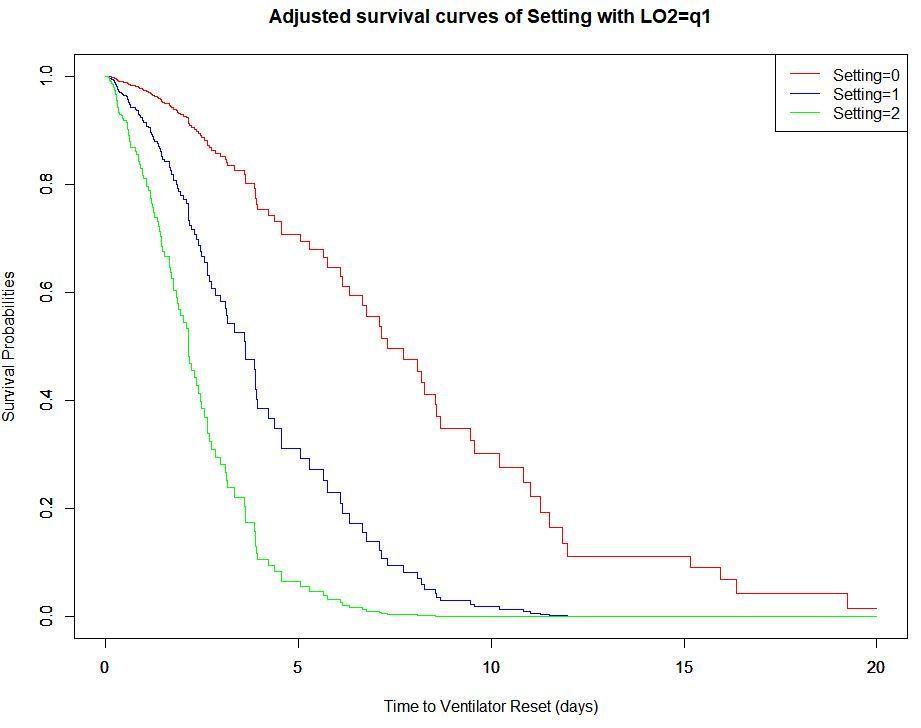
\includegraphics[width =10.5cm, height=7.5cm]{HW2AdjSurv.JPG}
\end{center}
\item Use the likelihood ratio test at $\alpha=0.05$ to test the significance of 
\begin{enumerate}[1.] 
\item Just Setting
\item  LO2 when Setting is in the model
 \item The interaction of LO2 and Setting when LO2 and Setting are in the model.
 \end{enumerate}
 In each case, compute the value of the test statistic and give the $p$-value of your test.
\end{enumerate}
\textbf{Problem 2}
A small study is conducted to test the effectiveness of a medication to treat alcohol dependence. The exposure variable is Dose in mg with 0 indicating the subject receives a placebo.   The response is time in weeks until alcohol consumption. The data below is collected on 7 subjects.
\begin{center}
\begin{tabular}{ c c c c } \hline
Subject & Time & Status & Dose \\ \hline
1 & 2 & 1 &  0\\
 2 & 3 & 0 &  1\\
3 & 5 & 0  & 0\\
4  & 6 & 1  & 1\\
5  & 6 & 1  & 1.5\\
6  & 7 & 1  & 2\\
7  & 8 & 1  & 1.5\\
\end{tabular}
\end{center}
Assume the Cox PH model and form the partial likelihood function. Maximize the function in R to find $\hat{\beta}$. Then make the data set in R and use the coxph routine to get the same estimate (note: this estimate might be slightly different because of the way that coxph handles ``ties''). What does $\hat{\beta}$ tell you about the effect of the dosage on the hazard of alcohol consumption? 

\end{document}  